\chapter{Background}
\lhead{Background}
\label{Background}

	The benthic habitat mapping technique and informative exploration policies devised in this thesis rely heavily on the inference framework of Gaussian processes. 
	
	In the outset of this chapter, Section \ref{Background:GaussianProcesses} motivates the advantages of Gaussian processes by discussing the general theory and framework of Gaussian process inference that are necessary for understanding the work in this thesis. The discussion begins with an introduction to Bayesian modeling in Section \ref{Background:GaussianProcesses:BayesianModeling}, where Gaussian processes are a non-parametric subclass thereof that provide high flexibility for Bayesian inference. The definition of Gaussian processes (definition \ref{Definition:GaussianRandomField}) then reveals the significance of kernel covariance functions, whose theory are then summarised in \ref{Background:GaussianProcesses:KernelFunctions}. The structure of Gaussian processes is then conveniently and readily applicable to standard regression problems, as demonstrated in Section \ref{Background:GaussianProcesses:Regression}, which also serves to motivate the way Gaussian processes are used for inference in general, which is further illustrated in \ref{Background:GaussianProcesses:Regression:GeneralGaussianProcessInferece}. The inference and learning stage involved in regression, formulated in sections \ref{Background:GaussianProcesses:Regression:Inference} and \ref{Background:GaussianProcesses:Regression:HyperparameterLearning} respectively, further outlines the specific way such an inference process works. Finally, the concept of entropy in differential and information forms are outlined in Section \ref{Background:GaussianProcesses:Entropy}, which forms the grounding for much of the acquisition techniques investigated and developed in this thesis.
	
	% The concepts involved here will then be reflected again in the techniques developed in this thesis for classification, whose basic structure and difficulties are explained in Section \ref{Background:GaussianProcesses:Classification}.
	
	Section \ref{Background:RelatedWork} then discusses the ways related work has approached the informative path planning problem using Gaussian processes, which stresses the . With a few examples of informative path planning techniques from Section \ref{Background:RelatedWork:InformativePathPlanning}, the importance of acquisition functions are stressed in Section \ref{Background:RelatedWork:AcquisitionFunctions} with reference to prior work.
	
	\section{Gaussian Processes}
	\label{Background:GaussianProcesses}
	
		Gaussian processes (GP) are stochastic processes which generalises the multi-variate Gaussian distribution. In a statistical learning and machine learning context, they are categorised as a type of \textit{supervised learning} method, which describes the problem of learning relationships between input and output variables from empirical data. The empirical data is also often referred to as the training set.
		
		Supervised learning methods are further categorised into regression and classification problems, depending on the nature of the output variable. The problem is a regression problem if the output is continuous, and a classification problem if the output is discrete. For example, seafloor depth or terrain modeling is a typical regression problem, in which the terrain elevation structure is the continuous output to be inferred. Benthic habitat mapping, on the other hand, involves inference of discrete habitat labels and is thus a classification problem.
		
		In both regression and classification settings, the input variables are often also referred to as \textit{features}, which motivated the term \textit{bathymetric features} in the previous sections. This also helps to distinguish the features from the spatial inputs, which are not necessarily the input variables involved in the supervised learning problem. In statistical literature, continuous regression outputs are sometimes called \textit{response} variables, although it is more often simply referred as the \textit{output} or \textit{target} in the machine learning community. However, in the Gaussian process classification setting, the term \textit{response} also refers to the likelihood response involved in the model. Therefore, the use of the term \textit{response} will be reserved for the latter in this thesis. Discrete classification outputs are often referred to as \textit{labels}, although the term \textit{target} is also used. In the benthic habitat mapping context, the type of henthic habitats are the labels to be inferred or predicted. 
		
		In the sections which references the use of Gaussian process models, $\bvec{x}$ will denote the input variable or features of the problem while $y$ will denote the output or target variable. Note that in general there are multiple features such that the input is a feature vector $\bvec{x}$. Without loss of generality, however, the output variable can always be treated as a scalar quantity $y$. Under cases of multiple output variables, the problem can be split into multiple single output variable problems.
		
		%%% If I need to talk about multi-task regressoin, put it in the appendix and put a note here saying that I can expand on this more.
		
		% It is true that prediction performance may be improved by considering the output vector together, which leads to multi-task regression, as will be briefly discussed. However, this is only the case if the training features the multiple outputs are located in different parts of the feature space, which does not occur for 

		The work presented here will be primarily based on \textit{Gaussian Process for Machine Learning} by \cite{GaussianProcessForMachineLearning}. 

		\subsection{Bayesian Modeling with Gaussian Processes}
		\label{Background:GaussianProcesses:BayesianModeling}
		
			The Gaussian process formulation follows the Bayesian modeling philosophy. An important distinction Bayesian modeling makes from the classical approach is the idea of estimating a distribution instead of a point value. While this is often more computationally expensive, it provides a very robust and accurate framework for prediction and inference. More importantly, it provides capabilities that classical approaches do not possess - the ability to quantify prediction uncertainties and, most importantly, potential information. 
			
			Suppose $H$ represents the event that a particular inference model $\mathcal{H}$ is representative of the true underlying phenomenon to be inferred. Further suppose $D$ represents the event that a particular set of observations $\mathcal{D}$ have been collected. The basic Bayesian modeling process begins with a \textit{prior} distribution $p(H)$, the probability of $\mathcal{H}$ being representative before $\mathcal{D}$ was observed, and updates this to a \textit{posterior} distribution $p(H | D)$, the updated probability of $\mathcal{H}$ being representative after observing $\mathcal{D}$. In this way, $\mathcal{H}$ can be interpreted as the agent's belief of the phenomenon. In benthic habitat mapping, the agent is the AUV, and the phenomenon is the type of benthic habitats distributed about the region of interest.
			
			In general, this belief update is achieved through Bayes theorem \eqref{Equation:Bayes}. The \textit{likelihood} distribution $p(D | H)$ is the probability of observing the dataset $\mathcal{D}$ given that $\mathcal{H}$ is representative of the true underlying phenomenon. The \textit{evidence} distribution $p(D)$ is the probability of observing the dataset in general. However, in practice it is often difficult to compute the evidence without a model. Hence, expanding over all possible inference models $\mathcal{H}$, the evidence can also be found by marginalising the joint distribution $p(D \cap H) = p(D | H) p(H)$ of observing $\mathcal{D}$ and $\mathcal{H}$ being representative. In this way, the evidence is also referred to as the \textit{marginal likelihood}. \begin{equation}
				p(H | D) = \frac{p(D | H) p(H)}{\underbrace{p(D)}_{\sum_{H} p(D | H) p(H)}} \qquad \Longleftrightarrow \qquad \mathrm{posterior} = \frac{\mathrm{likelihood} \times \mathrm{prior}}{\mathrm{evidence}}
			\label{Equation:Bayes}
			\end{equation} This procedure is illustrated in \cref{Figure:BayesianModeling} for a Gaussian process with one dimensional input feature and output target. The mean prediction is shown as the black solid curve. Ten sample functions from the GP are drawn from the prior (figure \ref{Figure:BayesianModeling:Prior}) and posterior (figure \ref{Figure:BayesianModeling:Posterior}), represented by the coloured dashed curve. The shaded region represents the 2-$\sigma$ bounds of the prediction at each input feature value $x$. The prior distribution is updated to a posterior distribution after two points are observed. This example further serves to illustrate the concept of distributions over functions, which behaves as an infinite dimensional generalisation of a multivariate probability distribution. It is helpful to conceptualise functions as an infinite string of points, where functions can be interpreted as infinite dimensional vectors, such that drawing from an infinite dimensional distribution is equivalent to drawing from processes that operate on function space. Instead of drawing finite dimensional random vectors from distributions, a random function is drawn from a \textit{stochastic process} \footnote{When the input variable is temporal, a stochastic process can be more appropriately interpreted as having indefinite dimensional distributions.}.
			
			\begin{figure}[!htbp]
			\centering
			  \subfigure[Prior distribution of functions]{\label{Figure:BayesianModeling:Prior}	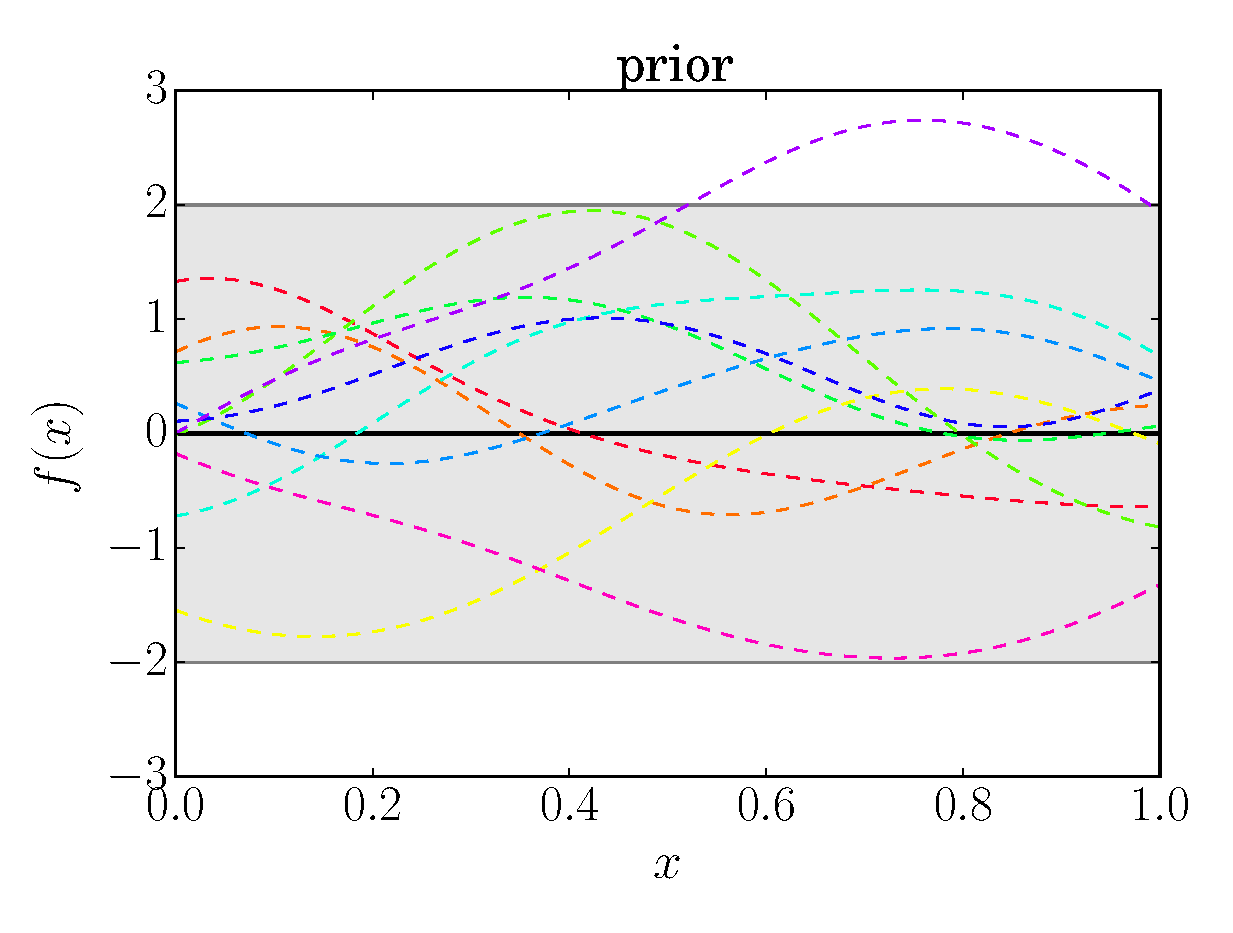
\includegraphics[width=0.48\linewidth]{Figures/bayesian_modeling/prior_draws.eps}}
			  \subfigure[Posterior distribution of functions]{\label{Figure:BayesianModeling:Posterior}	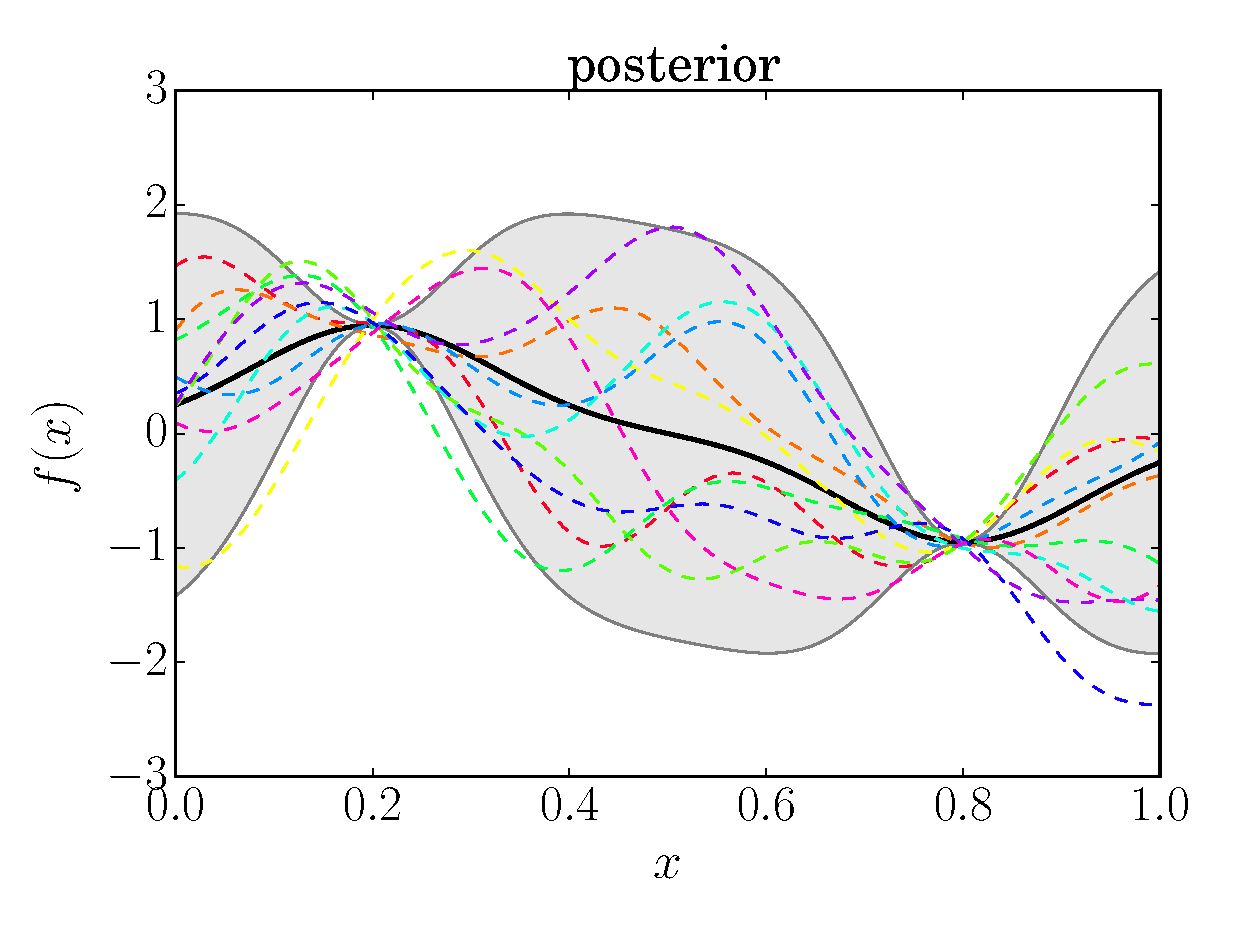
\includegraphics[width=0.48\linewidth]{Figures/bayesian_modeling/posterior_draws2.eps}}
			\caption{Illustration of Gaussian Process Bayesian Modeling}
			\label{Figure:BayesianModeling}
			\end{figure}
			
%			\begin{figure}[!htbp]
%				\centering
%					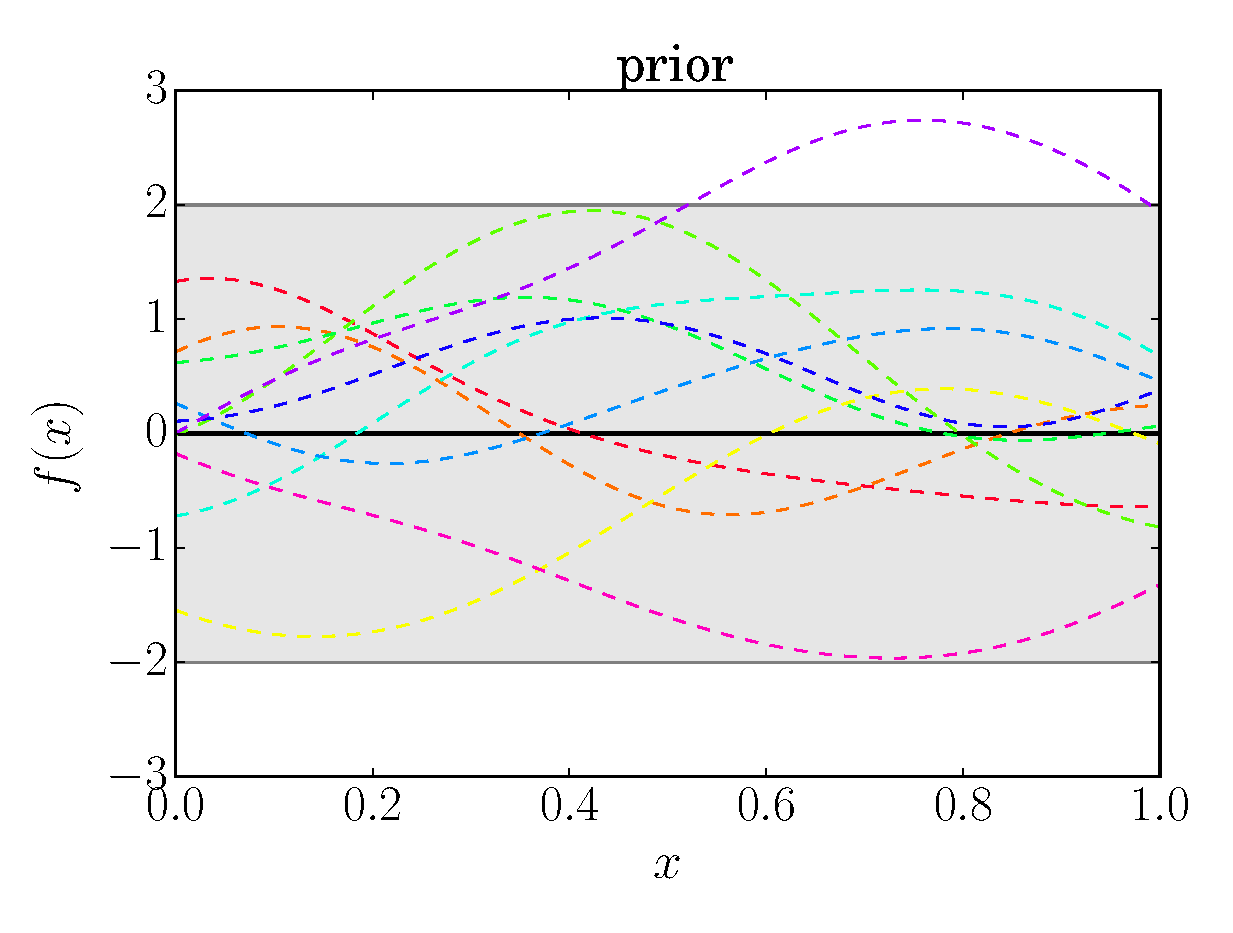
\includegraphics[width=0.48\textwidth]{Figures/bayesian_modeling/prior_draws.eps}
%					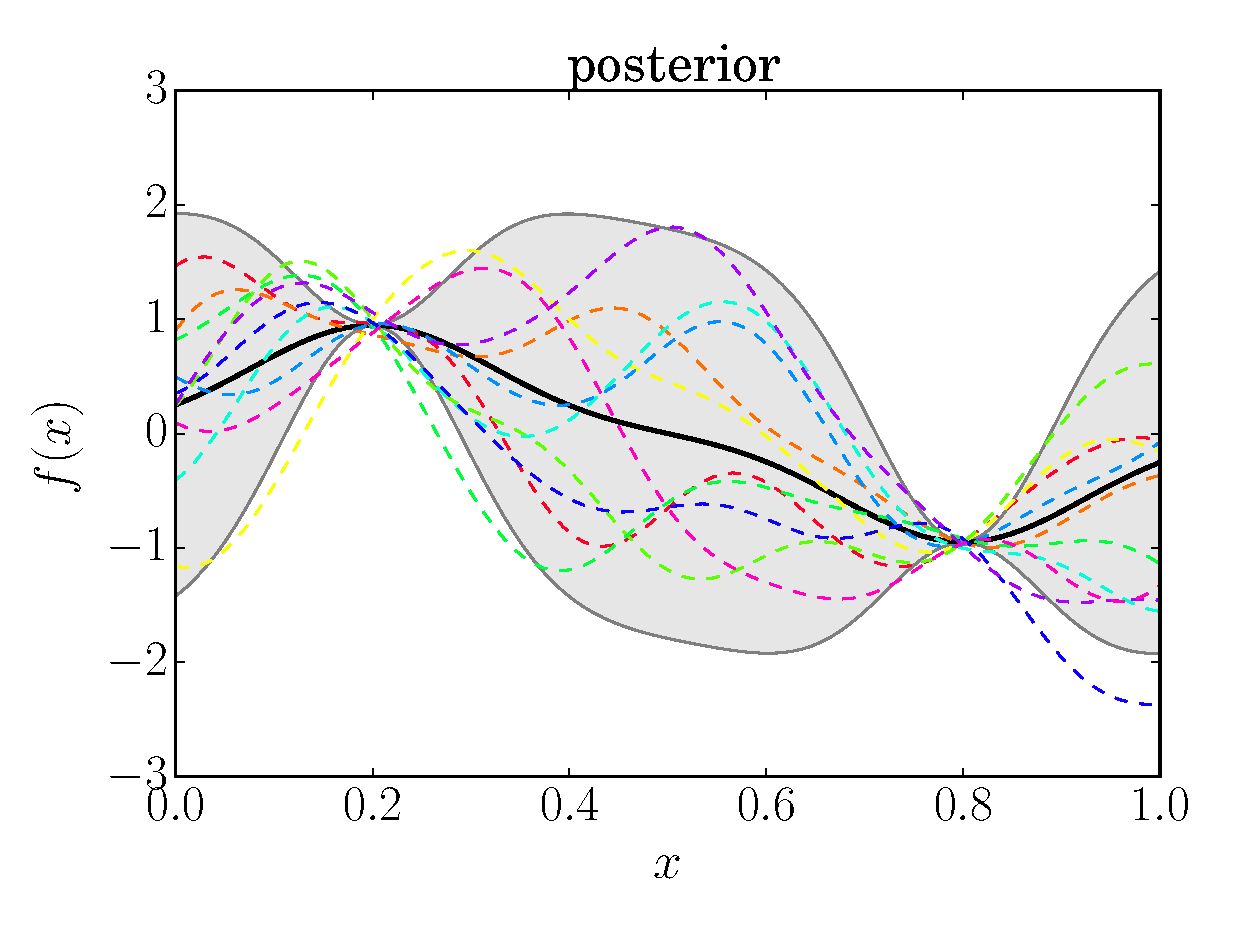
\includegraphics[width=0.48\textwidth]{Figures/bayesian_modeling/posterior_draws2.eps}
%				\caption{Illustration of Gaussian Process Bayesian Modeling}
%				\label{Figure:BayesianModeling}
%			\end{figure}
			
			From this illustration, there are a few qualities one can notice. Firstly, the prior distribution is simply the zero function. The prior is meant to represent the system's current belief before the next observations are to be made. In this case, the prior situation involves no observations at all. Ideally, this means that the prior distribution should contain no predictive information. However, it is of philosophical note that all informative \footnote{It is certainly possible to perform inference without any assumptions. It will simply be uninformative in prediction or result.} inferences must begin with some assumptions regarding the structure of the phenomenon to be inferenced. In the illustration above, the function is assumed to be distributed as a process with zero mean. This assumption has excluded processes without means, such as the Cauchy process, as well as assumed a rather arbitrary mean function. However, this assumption is often valid as one can always pre-process the output data set through subtracting off their empirical mean so that the output is approximately distributed about zero. The representation of the standard deviation and hence variance as confidence bounds centred at the mean function also means that multi-model processes are excluded. For a Gaussian process, which is indeed uni-modal and have finite moments for all moments of finite degree, this illustration is common and useful for visualising the Bayesian modeling process. It is customary to visualise the 2-$\sigma$ bound for a Gaussian process. So, for this example, the prior distribution has a uniform standard deviation of one everywhere.
			
			Regarding the variance, a second observation is that the standard deviation and hence variance of the output function decreases at the observations, and gradually increases away from the observations. This leads to two remarks. Firstly, the variance or uncertainty of the output function at a location reduces when observations are made at that location. Secondly, neighboring points are related - the closer they are, the more related they are. This is seen through the observed points dragging nearby points towards it while reducing the uncertainty of nearby points. This resembles the concept of covariance. 
%			Evidently, points closer to each other have higher covariance then those further away, and the covariance beween the same points simply become its variance.
			
			The two observations above demonstrate that, just as a Gaussian distribution is defined through a mean vector and a covariance matrix, a Gaussian process is defined through a mean function $m(x)$ and a covariance function $k(x, x')$. In Gaussian process literature, the covariance function is also called a \textit{kernel} function.
			
			With an intuition of Gaussian processes in the Bayesian modeling context, a formal definition of Gaussian processes can now be introduced. 
%			In this thesis, the shorthand notation $I_{n} := \{1, 2, \dots, n\}$ will be used for concise indexing unless otherwise indicated, and is not to be confused with identity matrices $I_{p \times p} \in \mathbb{R}^{p \times p}$.
			
%			\newpage
%			\newtheorem{gpdef}{Gaussian Process}[section]
%			\begin{gpdef}
%				A random function $f(x)$, $x \in \mathbb{R}$, is distributed as a Gaussian process with mean function $m(x)$ and covariance function $k(x, x')$, if for any finite collection of features $\bvec{x} := \{x_{i}\}_{i \in I_{n}} := [x_{1}, x_{2}, \dots, x_{n}]^{T}$, the corresponding vector $\bvec{f}(\bvec{x}) := \{f(x_{i})\}_{i \in I_{n}} := [f(x_{1}), f(x_{2}), \dots, f(x_{n})]^{T}$ is jointly multivariate Gaussian distributed such that \begin{equation}
%						\bvec{f}(\bvec{x}) \sim \mathcal{N}(\bvec{m}(\bvec{x}), K(\bvec{x}, \bvec{x}'))
%					\label{Equation:GaussianProcessFiniteDistribution}
%					\end{equation} where $\bvec{m}(\bvec{x}) :=  \{m(x_{i})\}_{i \in I_{n}} \in \mathbb{R}^{n}$ and $K(\bvec{x}, \bvec{x}') := \{k(x_{i}, x_{j})\}_{i \in I_{n}, j \in I_{n}}$. Such a function $f(x)$ is then notated as \begin{equation}
%						f(x) \sim \mathcal{GP}(m(x), k(x, x'))
%					\label{Equation:GaussianProcess}
%					\end{equation}	
%					
%			\label{Definition:GaussianProcess}
%			\end{gpdef}
%			
%			Certainly, this definition generalises finite dimensional multivariate Gaussian distributions, in that any subset of a multivariate Gaussian distributed random vector is also a multivariate Gaussian distributed of lower dimensionality.
%
%			Definition \ref{Definition:GaussianProcess} is defined for a univariate input feature $x$. In fact, this definition generalises naturally to a multivariate input feature $\bvec{x} \in \mathbb{R}^{p}$ with $p$ features. This motivates definition \ref{Definition:GaussianRandomField}.
			
			\newtheorem{grfdef}{Gaussian Process}[section]
			\begin{grfdef}
				A random function $f(\bvec{x})$, $\bvec{x} \in \mathbb{R}^{p}$, is distributed as a Gaussian process with mean function $m(\bvec{x})$ and covariance function $k(\bvec{x}, \bvec{x}')$, if for any finite collection of feature vectors $X := \{\bvec{x}_{i}\}_{i \in I_{n}}$, the corresponding vector $\bvec{f}(X) := \{f(\bvec{x}_{i})\}_{i \in I_{n}}$ is jointly multivariate Gaussian distributed such that \begin{equation}
						\bvec{f}(X) \sim \mathcal{N}(\bvec{m}(X), K(X, X'))
					\label{Equation:GaussianRandomFieldFiniteDistribution}
					\end{equation} where $\bvec{m}(X) :=  \{m(\bvec{x}_{i})\}_{i \in I_{n}} \in \mathbb{R}^{n}$ and $K(X, X') := \{k(\bvec{x}_{i}, \bvec{x}_{j})\}_{i \in I_{n}, j \in I_{n}}$. Such a function $f(\bvec{x})$ is then notated as \begin{equation}
						f(\bvec{x}) \sim \mathcal{GP}(m(\bvec{x}), k(\bvec{x}, \bvec{x}'))
					\label{Equation:GaussianRandomField}
					\end{equation}	
					
			\label{Definition:GaussianRandomField}
			\end{grfdef}
			
%			Definition \ref{Definition:GaussianRandomField} is defined for a general multivariate input feature $\bvec{x}$. Formally, a Gaussian process is a specific case of a Gaussian random field where the input feature $\bvec{x} = x$ is one dimensional. However, in practice the term ``Gaussian random field'' is seldom used, and instead are also referred to as Gaussian processes. As such, it is conventional to simply write $\mathcal{GP}$ instead of $\mathcal{GRF}$ in \eqref{Equation:GaussianRandomField}. Finally, as the mean function can be generally assumed to be the zero function, this elucidates that Gaussian processes are completely defined by their covariance function $k$. The covariance function $k$ is also refered to as the \textit{kernel} function.
			
%			Certainly, this definition generalises finite dimensional multivariate Gaussian distributions, in that any subset of a multivariate Gaussian distributed random vector is also a multivariate Gaussian distributed of lower dimensionality.
			
		\subsection{Kernel Functions}
		\label{Background:GaussianProcesses:KernelFunctions}

			As kernel functions completely define the inference characteristics of a Gaussian process, this section aims to provide the minimal mathematical background regarding kernels that are necessary for understanding Gaussian processes. 
			
			Intuitively, the kernel function determines the \textit{similarity} between data points. This is a notion that all supervised learning algorithms intend to do, although rather implicitly in most cases. The GP formulation makes this explicit through the covariance between any two points in the feature space.
			
			Kernel functions can be categorised into stationary kernels and non-stationary kernels. The work in this thesis only requires stationary kernels, which are much faster to compute than non-stationary kernels. The following discussion focuses on the stationary kernel functions used in this thesis. Other examples of stationary and non-stationary kernels are discussed in Appendix \ref{Appendix:CommonKernelFunctions}.
			
			Stationary kernels are ones whose covariance properties do not depend explicitly on the locations $\bvec{x}$ and $\bvec{x}'$ of consideration, but only on the difference $\bvec{x} - \bvec{x}'$ between them. Thus, the covariance properties are \textit{stationary}, or invariant, under translations in the feature space.
			
			Common stationary kernels are the squared exponential kernel \footnote{Squared exponential kernels are also sometimes called Gaussian kernels. However, in conversations it tends to create confusion between the probability density function $\phi(x)$ for Gaussian distributions and the covariance function $k(x, x')$ itself, so this term is avoided in this thesis.} and the \matern kernels, both of which belongs to the class of \textit{radial basis function} kernels. The squared exponential (SE) kernel between any two points $\bvec{x}, \bvec{x}' \in \mathbb{R}^{p}$ in the feature space with $p$ features has the following form \eqref{Equation:SquaredExponentialKernel}. \begin{equation}
				\left.
					\begin{aligned}
						k_{\mathrm{SE}}(\bvec{x}, \bvec{x}') &= \sigma_{f}^{2} \exp\Big(-\frac{1}{2}(\bvec{x} - \bvec{x}')^{T} \Sigma^{-1} (\bvec{x} - \bvec{x}')\Big) = \sigma_{f} \exp\Big(-\frac{1}{2} a^{2} \Big) \\
						\Sigma &= 	\begin{bmatrix}
										l_{1}^{2} & l_{12} & \dots & l_{1p} \\
										l_{21}^{2} & l_{2}^{2} & \dots & l_{2p} \\
										\vdots & \vdots  & \ddots & \vdots \\
										l_{p1}^{2} & l_{p2} & \dots & l_{p}^{2} \\
								  	\end{bmatrix}
					\end{aligned}
				\qquad \right.
			\label{Equation:SquaredExponentialKernel}
			\end{equation} Here, $\sigma_{f}$ is called the sensitivity, and determines the overall reference strength scale of the covariance function. The matrix $\Sigma$ is the length scale matrix, and determines the reference length scale and principle axis directions within the feature space. Like most quadratic forms, $\Sigma$ is required to be symmetric and positive definite. In particular, when $\Sigma$ is diagonal, the kernel is termed \textit{axis aligned}. When $\Sigma$ is proportional to an identity such that $\Sigma = l^{2} I_{p \times p}$, the kernel is termed \textit{isotropic}.
			
			The sensitivity parameter $\sigma_{f}$ and length scale parameters $l_{ij}$, $i, j \in {1, 2, \dots, m}$ with $l_{i} := l_{ii}$ completely contain the information of a squared exponential kernel. Unlike parametric models, however, while these parameters define the kernel directly, they define the GP model indirectly. Because of the multiple levels of relation from these parameters to the model, these parameters are termed \textit{hyperparameters} of the GP.
			
			In practice, it is often possible to pre-process the data by transforming the feature space so that an axis aligned kernel can be applied. The assumption imposed is that the principle axis directions are aligned with the feature space axis. In this case, the GP model is defined by $p + 1$ hyperparameters. Without the axis-aligned structure, the number of hyperparameters is $\frac{p(p + 1)}{2} + 1$.
			
			The above formulation suggests to define $a^{2} := (\bvec{x} - \bvec{x}')^{T} \Sigma^{-1} (\bvec{x} - \bvec{x}')$. This can be interpreted as the squared distance between $\bvec{x}$ and $\bvec{x}'$ under the warp defined by $\Sigma$. In particular, when the feature space is isotropic such that $\Sigma = l^{2} I_{p \times p}$, then $a = \frac{r}{l}$ where $r := +\sqrt{r^{2}}$, $l := +\sqrt{l^{2}}$, and $r^{2} = (\bvec{x} - \bvec{x}')^{T} (\bvec{x} - \bvec{x}')$. In fact, most stationary kernels are functions solely of $a^{2}$, or with the definition $a := +\sqrt{a^{2}}$, they are simply scalar functions of scalar inputs $a = a (\bvec{x}, \bvec{x'})$. This form also makes evident that the covariances between two points decreases monotonically as the distance between them increases - a property most kernel functions exhibit. In fact, this structure characterises the \textit{radial basis function} class of kernels, and is the primary type of kernel relevant to this thesis.
			
		\subsection{Regression}
		\label{Background:GaussianProcesses:Regression}
		
			Gaussian process regression is a regression technique that employs Gaussian processes as its inference model. Because Gaussian processes already operate on function spaces with continuous inputs and outputs, no extra pre-processing or transformations are needed. The bulk of the technique thus lies in learning the kernel function of the Gaussian process. Gaussian process regression is also called \textit{kriging} or Kolmogorov Wiener prediction when used for interpolating geospatial data in a geostatistics setting. This section attempts to summarise the important concepts regarding GP regression and how they work.
			
			Once a kernel is chosen, learning the kernel function becomes equivalent to learning the hyperparameters of the kernel. In this way, the Gaussian process model is defined completely by its hyperparameters $\vec{\uptheta}$. To make this fact explicit, the kernel function is sometimes notated as $k_{\vec{\uptheta}}$ instead. % , which are often only handful in quantity. % This illustrates that while its temporal complexity $\mathcal{O}(n^{3})$ is quite high, its spatial complexity and memory requirements are quite moderate at $\frac{m(m + 1)}{2} + 1 + n(m  + 1)$ real numbers, where $n(m  + 1)$ real numbers comes from the training data itself. % Minimally, after assuming a particular kernel functional form, the bulk of the model information is held by the data set itself. Especially in big data applications, unlike generalised linear models and neural networks whose information vector \footnote{The information vector is the vector of all parameters that defines the model.} is proportional to the number of basis functions employed, a Gaussian process model can have its information stored by a few hyperparameters.
			
			Before presenting the inference process for Gaussian process regression however, it is important to understand the way Gaussian processes are used in general for Bayesian inference, which applies to both regression and classification.
			
			\subsubsection{General Inference Process with Gaussian Processes}
			\label{Background:GaussianProcesses:Regression:GeneralGaussianProcessInferece}
			
				The Gaussian processes formulation from definition \ref{Definition:GaussianRandomField} provides an framework for inferring the behaviour of an unknown function $f(\bvec{x})$. In general, however, the output target does not have to be the functional outputs $f := f(\bvec{x})$. Instead, the output targets are some quantity $y$ which can be directly observed and recorded. The function $f$ serves as an intermediate step to infer $y$ from $\bvec{x}$, and in general cannot be directly observed. Therefore, it is often called the \textit{latent function}.
				
				% Define block styles
				\tikzstyle{line} = [draw, -latex']
				\tikzstyle{cloud1} = [draw, ellipse, fill = green!30!blue!30, node distance = 3cm, minimum height = 3em,  minimum width = 5em]
				\tikzstyle{cloud2} = [draw, ellipse, fill = green!60!blue!50, node distance = 3cm, minimum height = 3em,  minimum width = 5em]
				
				\begin{figure}[!ht]
				\centering\makebox[\textwidth]{
					\begin{tikzpicture}[node distance = 2cm, auto, comment/.style ={rectangle, inner sep = 2pt, text width = 4cm, }]
					
					\node [cloud1] (trainingfeatures) {$X$};
					\node [cloud2, right of = trainingfeatures] (traininglatents) {$\bvec{f}$};
					\node [cloud1, right of = traininglatents] (trainingtargets) {$\bvec{y}$};
					\node [cloud2, below of = traininglatents] (querylatents) {$\bvec{f}^{\star}$};
					\node [cloud1, left of = querylatents] (queryfeatures) {$X^{\star}$};
					\node [cloud2, right of = querylatents] (querytargets) {$\bvec{y}^{\star}$};
					
					\draw [line] (trainingfeatures) -- (traininglatents);
					\draw [line] (traininglatents) -- (trainingtargets);
					\draw [line] (traininglatents) -- (querylatents);
					\draw [line] (queryfeatures) -- (querylatents);
					\draw [line] (querylatents) -- (querytargets);	
					\end{tikzpicture}
					}		
				\caption{Gaussian Process Graphical Model}
				\label{Figure:GaussianProcessGraphicalModel}
				\end{figure}
				
				This inference process can be visualised with the graphical model presented in Figure \ref{Figure:GaussianProcessGraphicalModel}. The latent vectors $\bvec{f} = \{f(\bvec{x}_{i})\}_{i \in I_{n}}$ and $\bvec{f}^{\star} = \{f(\bvec{x}^{\star}_{i})\}_{i \in I_{n}}$ are defined in correspondence to the feature matrices $X = \{\bvec{x}_{i}\}_{i \in I_{n}}$ and $X^{\star} = \{\bvec{x}^{\star}_{i}\}_{i \in I_{n}}$, with $f$ as a random latent function distributed as a GP. Observed and known quantities are coloured in blue. Quantities to be inferred are coloured in green. Note that in a Bayesian model, the unknown quantities (in green) are inferenced by their probabilistic distributions, and not just their estimated values. 
				
%				\begin{align*} \numberthis\label{Equation:TrainingQueryFeatureMatrices}
%					X &= \{\bvec{x}_{i}\}_{i \in I_{n}} \qquad & X^{\star} &= \{\bvec{x}^{\star}_{i}\}_{i \in I_{n}} \\
%					\bvec{f} &= \{f(\bvec{x}_{i})\}_{i \in I_{n}} \qquad & \bvec{f}^{\star} &= \{f(\bvec{x}^{\star}_{i})\}_{i \in I_{n}}
%				\end{align*}
				
				Latent functions are usually interpreted as the underlying phenomenon which stochastically generates the target outputs $y$.  The model assumes that a particular phenomenon $f$ is responsible for generating the output target $y$, and that the phenomenon $f$ can be explained reasonably by a particular set of features $\bvec{x}$. A collection of output targets $\bvec{y}$ and corresponding features $X$ are observed. The collected dataset $(X, \bvec{y})$ is termed the \textit{training data}. A \textit{learning process} then occurs where the model learns the underlying phenomenon $\bvec{f}$ at the training points. If the learning process is done through an optimisation procedure in search for an optimal model in some quantifiable sense, the learning process is also termed a \textit{training process}. An \textit{inference process} then occurs where the model is to infer the latent process $\bvec{f}^{\star}$ at the query features $X^{\star}$, which would further allow inference on the corresponding target outputs $\bvec{y}^{\star}$. The inference process in general also includes the act of inferring related quantities regarding the distribution of $\bvec{y}^{\star}$. Typical examples include inferring the uncertainty involved in the inference stage through a variance or entropy measure. If the only quantity to be inferenced is the expected target outputs $\mathbb{E}[\bvec{y}^{\star} | \bvec{y}, X, X^{\star}]$, then the inference process is also termed a \textit{prediction process}. In this way, the GP modeling process is composed of two stages - the learning or training stage and the inference or prediction stage.
				
				For regression, a typical example involves observable outputs $y$ that are related to the underlying phenomenon $f$ through a simple white noise process \eqref{Equation:RegressionNoiseModelScalar}, where $\sigma \geq 0$ is the standard deviation of the \textit{iid} zero mean Gaussian distributed noise. \begin{equation}
					y_{i} = f(\bvec{x}_{i}) + \epsilon_{i} \qquad \epsilon_{i} \sim \mathcal{N}(0, \sigma^{2}) \qquad \mathrm{iid} \qquad \forall i \in I_{n}
				\label{Equation:RegressionNoiseModelScalar}
				\end{equation} In general, however, the relationship between the output target $y$ and the latent functional $f$ is captured through a \textit{likelihood response} $p(y | f)$, the probability of generating a particular output target $y$ \textit{if} the latent functional is $f$. In fact, the choice of the likelihood function is not immediately straightforward and is of vital importance in the classification scenario. 
				
				In the regression model above \eqref{Equation:RegressionNoiseModelScalar}, a degenerate case arises when the noise level $\sigma$ is zero such that $y = f$ everywhere. In this case, $p(y | f) = p(f | f) = 1$ such that the Gaussian process model performs inference on the target output directly through obtaining $p (y) = p(f)$. When this is not the case, however, the quantity to be inferred in the end is the output targets $y$. As such, the distribution of interest is $p(y)$. This can be obtained by marginalising away the latent functionals $f$ over the likelihood $p(y | f)$ \eqref{Equation:Marginalisation} where $\mathscr{F}$ is the space of all latent functionals. \begin{equation}
					p(y) = \int_{\mathscr{F}} p(y | f) p(f) df
				\label{Equation:Marginalisation}
				\end{equation}
				
%				Note that the form \eqref{Equation:Marginalisation} above is written in functional form to illustrate the relevant concepts. The marginalisation process above plays a vital process in the learning stage for Gaussian process inference discussed shortly.
		
			\subsubsection{Inference}
			\label{Background:GaussianProcesses:Regression:Inference}
			
				The above inference process can now be formulated specifically for regression. The inference stage assumes that the hyperparameters $\vec{\uptheta}$ has been learned, which allows the distribution of $\bvec{f} | \vec{\uptheta}, \bvec{y}$ to be specified from the observations $\bvec{y}$. This allows inference through correlation for $\bvec{f}^{\star} | \bvec{f}, \vec{\uptheta}$ and finally $\bvec{y}^{\star} | \bvec{f}^{\star}, \vec{\uptheta}$ through a likelihood response (figure \ref{Figure:GaussianProcessGraphicalModel}). An understanding of such an inference process will motivate the discussion of the hyperparameter learning stage in the following section.
				
				With a given kernel function $k = k_{\vec{\uptheta}}$ as the covariance function, by definition \ref{Definition:GaussianRandomField} we have that the training latents $\bvec{f}$ at training features $X$ and the query latents $\bvec{f^{\star}}$ at query features $X^{\star}$ are distributed as a multivariate Gaussian \eqref{Equation:InferenceJointDistribution}. To shorten notation, it is customary to define the following kernel matrices \eqref{Equation:KernelMatrices}, where the symmetry of covariance matrices readily yields $K_{\vec{\uptheta}}(X^{\star}, X) = {K_{\vec{\uptheta}}^{\star}}^{T}$. In this thesis, $K \in \mathbb{R}^{n \times n}$ will be referred to as the \textit{data kernel} or \textit{training kernel}, $K^{\star} \in \mathbb{R}^{n \times n^{\star}}$ as the \textit{inference kernel}, and $K^{\star \star} \in \mathbb{R}^{n^{\star} \times n^{\star}}$ as the \textit{query kernel}. \begin{equation}
					\begin{bmatrix}
						\bvec{f} \\ \bvec{f}^{\star}
					\end{bmatrix} \Bigg|_{\vec{\uptheta}}
					\sim \mathcal{N}\Bigg(\bvec{0}, \begin{bmatrix}
														K_{\vec{\uptheta}}(X, X) & K_{\vec{\uptheta}}(X, X^{\star}) \\
														K_{\vec{\uptheta}}(X^{\star}, X) & K_{\vec{\uptheta}}(X^{\star}, X^{\star}) \\
													\end{bmatrix}  \Bigg)
				\label{Equation:InferenceJointDistribution}
				\end{equation} \begin{equation}
					\begin{aligned}
						& K = K_{\vec{\uptheta}} := K_{\vec{\uptheta}}(X, X) := \{k_{\vec{\uptheta}}(\bvec{x}_{i}, \bvec{x}_{j})\}_{i \in I_{n}, j \in I_{n}} \\
						& K^{\star} = K_{\vec{\uptheta}}^{\star} := K_{\vec{\uptheta}}(X, X^{\star}) := \{k_{\vec{\uptheta}}(\bvec{x}_{i}, \bvec{x}^{\star}_{j})\}_{i \in I_{n}, j \in I_{n^{\star}}} \\
						& K^{\star \star} = K_{\vec{\uptheta}}^{\star \star} := K_{\vec{\uptheta}}(X^{\star}, X^{\star}) := \{k_{\vec{\uptheta}}(\bvec{x}^{\star}_{i}, \bvec{x}^{\star}_{j})\}_{i \in I_{n^{\star}}, j \in I_{n^{\star}}}
					\end{aligned}
				\label{Equation:KernelMatrices}
				\end{equation} The joint distribution readily contains information for the conditional distribution of the query points given the training points $p(\bvec{f^{\star}} | \bvec{f}, \vec{\uptheta})$ knowing the training points and query locations. This leads to the posterior distribution \eqref{Equation:InferencePosteriorLatentDistribution}. Note that in some literature, the features $X$ and $X^{\star}$ are also included in the conditioned set, so that the conditional distribution is written as $\bvec{f^{\star}} | \bvec{f}, \vec{\uptheta}, X, X^{\star}$. However, all relevant information required in the inference stage from $X$ and $X^{\star}$ is summarised by the hyperparameters $\vec{\uptheta}$ given a particular kernel function. Hence, they are always inherently conditioned upon and will not be shown explicitly in notation for consise presentation in this thesis. \begin{equation}
					\bvec{f^{\star}} | \bvec{f}, \vec{\uptheta} \sim \mathcal{N}({K_{\vec{\uptheta}}^{\star}}^{T} K_{\vec{\uptheta}}^{-1} \bvec{f}, K_{\vec{\uptheta}}^{\star \star} - {K_{\vec{\uptheta}}^{\star}}^{T} K_{\vec{\uptheta}}^{-1} K_{\vec{\uptheta}}^{\star})
				\label{Equation:InferencePosteriorLatentDistribution}
				\end{equation} A comparison with the prior $\bvec{f^{\star}} | \vec{\uptheta} \sim \mathcal{N}(\bvec{0}, K_{\vec{\uptheta}}^{\star \star})$ shows the mean effect ${K_{\vec{\uptheta}}^{\star}}^{T} K_{\vec{\uptheta}}^{-1} \bvec{f}$ and covariance effect $- {K_{\vec{\uptheta}}^{\star}}^{T} K_{\vec{\uptheta}}^{-1} K_{\vec{\uptheta}}^{\star}$ which introduces observed information into the model. Interestingly, as ${K_{\vec{\uptheta}}^{\star}}^{T} K_{\vec{\uptheta}}^{-1} K_{\vec{\uptheta}}^{\star}$ is positive definite, this intuitively means that the observation has reduced uncertainty in the model. The above posterior distribution encompasses the heart of the GP regression model. The rest of the discussion will focus on detailed aspects of its implementation and variants.
				
				As in the case of \eqref{Equation:RegressionNoiseModelScalar}, if the noise $\sigma$ is zero such that the output target $y$ degenerates to the latent $f$, then the predictive distribution $\bvec{y^{\star}} | \bvec{y}, \tilde{\vec{\uptheta}}$ is also the latent posterior distribution \eqref{Equation:InferencePosteriorLatentDistribution}, so that all inferences required can be obtained from the posterior. Under noisy observations with $\sigma > 0$ however, $\sigma$ is introduced as a hyperparameter so that the hyperparameters becomes $\tilde{\vec{\uptheta}} := [\vec{\uptheta}, \sigma]^{T}$, and the posterior distribution becomes \eqref{Equation:InferencePosteriorDistribution}. This is done by marginalising away $\bvec{f}$ through \eqref{Equation:MarginalisingLatent} where $p(\bvec{f^{\star}} | \bvec{f}, \tilde{\vec{\uptheta}})$ is from the latent posterior distribution \eqref{Equation:InferencePosteriorLatentDistribution} and $p(\bvec{f} | \bvec{y}, \tilde{\vec{\uptheta}})$ is specified by \eqref{Equation:TrainingPosterior} as a straightforward consequence from \eqref{Equation:RegressionNoiseModelScalar}, which effectively replaces the data kernel $K_{\vec{\uptheta}}$ with $B_{\tilde{\vec{\uptheta}}} := K_{\vec{\uptheta}} + \sigma^{2} I$, where $I := I_{n \times n}$, and thus incorporates the noise in the training data into the model. Finally, to find the predictive distribution for $\bvec{y^{\star}} | \bvec{y}, \tilde{\vec{\uptheta}}$, it suffices to add the noise variance to the posterior distribution \eqref{Equation:InferencePredictiveDistribution}. \begin{equation}
					p(\bvec{f^{\star}} | \bvec{y}, \tilde{\vec{\uptheta}}) = \int_{\mathbb{R}^{n}} p(\bvec{f^{\star}} | \bvec{f}, \tilde{\vec{\uptheta}}) p(\bvec{f} | \bvec{y}, \tilde{\vec{\uptheta}}) d\bvec{f}
				\label{Equation:MarginalisingLatent}
				\end{equation} \begin{equation}
					\bvec{f} | \bvec{y}, \tilde{\vec{\uptheta}} \stackrel{\bvec{f} | \bvec{y}, \sigma \perp \vec{\uptheta}}{=} \bvec{f} | \bvec{y}, \sigma \sim \mathcal{N}(\bvec{y}, \sigma^{2} I)
				\label{Equation:TrainingPosterior}
				\end{equation} \begin{equation}
					\bvec{f^{\star}} | \bvec{y}, \tilde{\vec{\uptheta}} \sim \mathcal{N}({K_{\vec{\uptheta}}^{\star}}^{T} (K_{\vec{\uptheta}} + \sigma^{2} I)^{-1} \bvec{y}, K_{\vec{\uptheta}}^{\star \star} - {K_{\vec{\uptheta}}^{\star}}^{T} (K_{\vec{\uptheta}} + \sigma^{2} I)^{-1} K_{\vec{\uptheta}}^{\star})
				\label{Equation:InferencePosteriorDistribution}
				\end{equation} \begin{equation}
					\bvec{y^{\star}} | \bvec{y}, \tilde{\vec{\uptheta}} \sim \mathcal{N}({K_{\vec{\uptheta}}^{\star}}^{T} (K_{\vec{\uptheta}} + \sigma^{2} I)^{-1} \bvec{y}, K_{\vec{\uptheta}}^{\star \star} + \sigma^{2} I_{n^{\star} \times n^{\star}} - {K_{\vec{\uptheta}}^{\star}}^{T} (K_{\vec{\uptheta}} + \sigma^{2} I)^{-1} K_{\vec{\uptheta}}^{\star})
				\label{Equation:InferencePredictiveDistribution}
				\end{equation}
								
			\subsubsection{Hyperparameter Learning}
			\label{Background:GaussianProcesses:Regression:HyperparameterLearning}
			
				One of the most important yet tricky aspects of GP modeling is the training stage. Since the model is determined entirely by the hyperparameters, the hyperparameters must be optimised in accordance to some fitness metric. The fitness metric employed to be maximised is the marginal likelihood, otherwise termed as evidence, of the observed data. This is usually non-trivial to compute and, in most cases, analytical forms do not exist. Fortunately, due to the Gaussian structure of the GP model, there exists an analytical form for the marginal likelihood. In practice, however, it is computationally faster to compute the log marginal likelihood for optimisation \eqref{Equation:RegressionLogMarginalLikelihood}. Note that the hyperparameters includes the kernel sensitivity $\sigma_{f}$, the kernel length scales $\{l_{ij}\}_{i \in I_{p}, j \in I_{p}}$, and the noise level $\sigma$ if noise exists. That is, the hyperparameters to be optimised is $\vec{\uptheta}$ under noiseless regression and $\tilde{\vec{\uptheta}}$ under noisy regression. \begin{equation}
					\begin{aligned}
						\tilde{\vec{\uptheta}}_{\mathrm{opt}} &= \argmax_{\tilde{\vec{\uptheta}}} \log(p(\bvec{y} | \tilde{\vec{\uptheta}})) \\
						\log(p(\bvec{y} | \tilde{\vec{\uptheta}})) = - \frac{1}{2} \bvec{y}^{T} (K_{\vec{\uptheta}} + &\sigma^{2} I)^{-1} \bvec{y} - \frac{1}{2} \log|K_{\vec{\uptheta}} + \sigma^{2} I| - \frac{n}{2} \log(2 \pi)
					\end{aligned}
				\label{Equation:RegressionLogMarginalLikelihood}
				\end{equation} Note that the data kernel $K_{\vec{\uptheta}}$ is a function of $\vec{\uptheta}$ only, which contains all hyperparameters except for $\sigma$. It is important to understand that the marginal likelihood here refers to the evidence $p(\bvec{y} | \tilde{\vec{\uptheta}})$ of the following Bayes relation \eqref{Equation:RegressionLogMarginalLikelihoodBayes}. \begin{equation}
					p(\bvec{f} | \bvec{y}, \tilde{\vec{\uptheta}}) = \frac{p(\bvec{y} | \bvec{f}, \tilde{\vec{\uptheta}}) p(\bvec{f} | \tilde{\vec{\uptheta}})}{p(\bvec{y} | \tilde{\vec{\uptheta}})}
				\label{Equation:RegressionLogMarginalLikelihoodBayes}
				\end{equation} That is, the entire Bayes relation is conditioned on the hyperparameters $\tilde{\vec{\uptheta}}$, and the marginalised quantity is the latents $\bvec{f}$ \eqref{Equation:GeneralMarginalLikelihood}. \begin{equation}
					p(\bvec{y} | \tilde{\vec{\uptheta}}) = \int_{\mathbb{R}^{n}} p(\bvec{y} | \bvec{f}, \tilde{\vec{\uptheta}}) p(\bvec{f} | \tilde{\vec{\uptheta}}) d\bvec{f}
				\label{Equation:GeneralMarginalLikelihood}
				\end{equation} In practice, hyperparameter learning can be sped up by employing the fact that $\frac{1}{2} \log|K + \sigma^{2} I| = \frac{1}{2} \log|B| = \sum_{i} L_{ii} = \mathrm{trace}(L)$ for the first term in \eqref{Equation:RegressionLogMarginalLikelihood}, where $L$ is the Cholesky decomposition of $B$. Furthermore, the Cholesky decomposition $L$ leads to better numerical stability when inverting the matrix $B$ since $B = LL^{T}$ so that $B \backslash \bvec{y} = L^{T} \backslash (L \backslash \bvec{y})$ for the first term in \eqref{Equation:RegressionLogMarginalLikelihood}. The last term in \eqref{Equation:RegressionLogMarginalLikelihood} is a constant, so it can be ignored during the optimisation stage.
				
%				Again, in the degenerate case where $y = f$ everywhere so that $\sigma = 0$ in \eqref{Equation:RegressionLogMarginalLikelihood}, the objective simply becomes the prior $p(\bvec{f} | \tilde{\vec{\uptheta}}) = p(\bvec{f} | \vec{\uptheta})$.
				
		\subsection{Entropy}
		\label{Background:GaussianProcesses:Entropy}
		
			In either the regression and classification case, after a predictive probability distribution for $\bvec{y}^{\star}$ is obtained for each query feature location, a prediction $\mathbb{E}[\bvec{y}^{\star}]$ can be obtained. Nevertheless, the power of a Bayesian model lies with its ability to also quantify prediction uncertainties. In this thesis, \textit{entropy} is employed as the measure of uncertainty and information which enables the process of informative path planning. Below discusses the entropy of general probability distributions.
			
			Specifically, the \textit{entropy} of a probability distribution is the expected amount of information or unpredictability contained in a distribution \citep{ShannonEntropy}. While the variance $\mathbb{V}[\bvec{y}^{\star}]$ is a perfectly valid way to quantify uncertainty, it is usually measured in the squared unit of the quantity interested. On the other hand, entropy is always measured in nats. More importantly however is the fact that entropy directly measures the amount of information to be expected from the query locations, such that informative actions can be taken.
			
			For a random vector $\bvec{X} \in A$ with continuous support $A$ and a probability density function $p(\bvec{x})$, the entropy is called a \textit{differential entropy}. On the other hand, for a random vector $\bvec{X} \in B$ with discrete support $B$ and a probability mass function $p(\bvec{x})$, the entropy is called a \textit{information entropy}. \begin{equation}
				H(\bvec{X}) = - \int_{A} p(\bvec{x}) \log(p(\bvec{x})) d\bvec{x} \qquad H(\bvec{X}) = - \sum_{\bvec{x} \in B} p(\bvec{x}) \log(p(\bvec{x})) d\bvec{z}
			\label{Equation:Entropy}
			\end{equation} The above notation is used in most statistics literature. However, in the machine learning context where the training features $X$ and targets $\bvec{y}$ are observed and the query targets $\bvec{y}^{\star}$ corresponding to query features $X$ are to be inferred, it is customary to write $H(\bvec{y}^{\star}) \equiv H[X^{\star} | X, \bvec{y}]$, which is understood as the ``entropy of the targets $\bvec{y}^{\star}$ at the query locations $X^{\star}$ given the observations $(X, \bvec{y})$''.

	\section{Related Work}
	\label{Background:RelatedWork}
		
		This section discusses the related work and approaches in the field of informative path planning. Section \ref{Background:RelatedWork:InformativePathPlanning} provides an overview of general informative path planning schemes, while Section \ref{Background:RelatedWork:AcquisitionFunctions} focuses on various acquisition functions that has been employed in the past to measure information.
				
		\subsection{Informative Path Planning}
		\label{Background:RelatedWork:InformativePathPlanning}
			
			Path planning under dynamic uncertainty has been a challenging task for all information searching missions. The objective is to maximised gathered information of a particular region under a particular resource, usually time, constraint. Unlike usual path planning scenarios, the information objective to be minimised throughout the path is not static as the vehicle make observations. Furthermore, this class of problems usually have no natural goal location, as reaching a particular destination is not the aim, although it can be artificially imposed if required.
		
			In an unmanned aerial vehicle setting, \cite{Roman:BayesianOptimisation} proposes a Bayesian Optimisation (BO) techniques combined with Gaussian process models for environmental monitoring. In this layered Bayesian Optimisation approach, two Gaussian processes are used - one to model the phenomenon and the other to model the quality of selected paths. Through Bayesian optimisation, sampling over continuous paths are optimised which maximises the reward over the final mission trajectory. The path planning process employs Markov Decision Processes (MDP) with a reinforcement learning approach. Rapidly Exploring Random Graphs (RRGs) is combined with BO to search for informative and continuous paths. This was was further extended for online path planning with Partially Observable Markov Decision Processes (POMDPs) using a Sequential Bayesian Optimisation (SBO) approach \citep{Roman:SequentialBayesianOptimisation}.
			
			In an autonomous underwater vehicle context, \cite{ParametricPOMDP} investigates a policy for continuous state space planning using POMDP. This work was compared to previous work with value-based and gradient-based solution methods which seek to transcribe the continuous problem into a discrete problem. One of the most important limitations is that analytical and accurate solutions exist almost only for linear systems with quadratic cost, or \textit{linear quadratic systems}. Otherwise, other options with non-value based methods require heuristics that can be difficult to justify for its appropriateness to the problem. 
			
			As such, informative path planning schemes often suffer from difficult tractability limitations as well as performance limitations due to the several levels of approximations or heuristics involved.
		
		\subsection{Acquisition Functions}
		\label{Background:RelatedWork:AcquisitionFunctions}
		
			One of the main challenges of informative path planning include selecting the appropriate acquisition function suitable for the type of exploration task at hand. \textit{Acquisition function}, or \textit{acquisition criterion}, measures the desirability of observing a particular location. In the informative path planning scenario, the acquisition function evaluates the amount of total information or uncertainty contained by a given candidate path. In this context, the way in which \textit{total information} is quantified determines the acquisition function. The more informative the path, the more desirable it is for the AUV to follow and take observations there.
	
			%\citep{AsherBender, Rigby:ROB20372, Krause:2008:NSP:1390681.1390689, Kapoor}
			The effectiveness of an acquisition function that measures mutual information throughout a particular given path has been thoroughly investigated in the literature. \textit{Mutual information} refers to a measure of information that takes into account the overlapping information within the region or path in consideration. In most spatial sampling contexts, it is unlikely that two given locations within a region or path are completely unrelated or uncorrelated. Observations in one location provides partial information regarding other locations. Without considering mutual information, an agent such as an AUV may be prompted to observe locations that contain similar information, thus achieving inefficient mapping. %, which is the primary reason that an benthic habitats throughout a seafloor region can be mapped obtained without visiting all locations within the region exhaustively. 
			
			Several types of acquisition functions have been proposed in the benthic habitat mapping context. \cite{AsherBender} uses an acquisition criterion given by \eqref{Equation:AMPIE} where $\pi^{c}_{i}$ is the probability of the habitat label being a member of class $c \in I_{n_{C}}$ at query location $\bvec{x}^{\star}_{i}$ where $i \in I_{n^{\star}}$. Here $n_{C}$ is the number of classes and $n^{\star}$ is the number of query points. Again the query locations are denoted as $X^{\star} := \{\bvec{x}^{\star}_{i}\}_{i \in I_{n^{\star}}}$. \begin{equation}
				H_{\mathrm{AMPIE}} \stackrel{\text{abbrev.}}{:=} H_{\mathrm{AMPIE}}[X^{\star} | X, \bvec{y}] = - \frac{1}{n^{\star}} \sum_{i = 1}^{n^{\star}} \sum_{c = 1}^{n_{C}} \pi^{c}_{i} \log(\pi^{c}_{i})
			\label{Equation:AMPIE}
			\end{equation} For a given query point $i$, $- \sum_{c = 1}^{n_{C}} \pi^{c}_{i} \log(\pi^{c}_{i})$ is exactly the prediction information entropy $\{H_{\mathrm{PIE}}\}_{i} \stackrel{\text{abbrev.}}{:=} H_{\mathrm{PIE}}[\bvec{x}^{\star}_{i} | X, \bvec{y}] = - \sum_{c = 1}^{n_{C}} \pi^{c}_{i} \log(\pi^{c}_{i})$ at location $i \in I_{n^{\star}}$, which captures the local model uncertainty and thus potential information. As a result, the acquisition criterion given in \eqref{Equation:AMPIE} is the average of the marginalised prediction information entropy across query points, which does not capture mutual information through considering the joint distributions of the class labels across the set of query points $X^{\star}$. The term \textit{marginalised} emphasizes this fact. This acquisition criterion will thus be referred to as AMPIE for average marginalised prediction information entropy. In this approach, the quality of a given proposed path $X_{p}$ is assessed by an informative acquisition criterion $I[X_{p} | X, \bvec{y}, X_{s}]$, which is the difference of the AMPIE before and after an observation is made \eqref{Equation:AsherBenderAcquisitionCriterion} \citep{Rigby:ROB20372}. This utility is used in conjunction with a GP classifier under probabilistic least squares approximation to optimise selected survey paths through considering the differential entropy across the entire region of interest (ROI). Below, ($X, \bvec{y}$) are the already observed feature locations and habitat labels used for training as usual, $X_{s}$ is the set of query points representing the entire seafloor, and ($X_{p}, \bvec{y}_{p}$) are the features and labels of the proposed path. Note that before the path is traversed $\bvec{y}_{p}$ is a random vector. \begin{equation}
				I[X_{p} | X, \bvec{y}, X_{s}] = H_{\mathrm{AMPIE}}[X_{s} | X, \bvec{y}] - H_{\mathrm{AMPIE}}[X_{s} | X \cup X_{p}, \bvec{y} \cup \mathbb{E}[\bvec{y}_{p}]]
			\label{Equation:AsherBenderAcquisitionCriterion}
			\end{equation} \cite{Krause:2008:NSP:1390681.1390689} instead focuses on sensor placement methodologies to optimse mutual information gained. This aims to reduce predictive variance at all query points. The chosen acquisition function is the difference between the AMPIE at all \textit{final} unobserved locations $X_{s} \backslash X_{p} := \big\{\bvec{x}^{\star} \big| \{\bvec{x}^{\star} \in X_{s}\} \cap \{\bvec{x}^{\star} \notin X_{p}\} \big\}$ before and after the observations are taken \eqref{Equation:KrauseAcquisitionCriterion}. \begin{equation}
				I[X_{p} | X, \bvec{y}, X_{s}] = H_{\mathrm{AMPIE}}[X_{s} \backslash X_{p} | X, \bvec{y}] - H_{\mathrm{AMPIE}}[X_{s} \backslash X_{p} | X \cup X_{p}, \bvec{y} \cup \mathbb{E}[\bvec{y}_{p}]]
			\label{Equation:KrauseAcquisitionCriterion}
			\end{equation} Under the GP classification model, however, this results in an integral that can only be estimated through sampling techniques which are computationally expensive. As such, computationally tractable methods usually employ experimental design philosophies in minimising the predictive variance \citep{AsherBender}.
			
			\cite{Kapoor} demonstrates the use of posterior mean and covariance of the GP classifier latent function. While this approach takes full advantage of the analytical forms available for a Gaussian latent process, it does not consider the mutual behaviour of the unobserved locations with the proposed path. On the other hand, while promising, the layered Sequential Bayesian Optimisation approach devised by \cite{Roman:SequentialBayesianOptimisation} is primarily devised for a regression setting which becomes difficult to emulate in the classification domain.
		
			Much of the intractability discussed in such literature can trace its reason down to the fact that benthic habitat mapping is a classification problem instead of a regression problem. While Gaussian process regression provide analytical forms for inference, due to a non-Gaussian likelihood response, Gaussian process classification is no longer analytically tractable.
			
			This thesis addresses the tractability status of the problem through proposing two alternative acquisition functions. In the current literature, acquisition criterion either do not directly capture mutual information, such as \eqref{Equation:AsherBenderAcquisitionCriterion}, or take too long to compute due to required estimations from sampling, such as \eqref{Equation:KrauseAcquisitionCriterion}. This work shows that the proposed acquisition functions improve both tractability and mapping accuracy.